\documentclass[11pt]{article}
\usepackage[margin=1in]{geometry}
\usepackage{siunitx}
\usepackage[version=4]{mhchem}
\usepackage{xltabular}
\usepackage{ragged2e}
\usepackage[font=small, skip=3pt, labelfont=bf]{caption}
\usepackage{float}
\usepackage{amsmath}
\usepackage{multirow}
\usepackage{enumitem}

\DeclareSIUnit{\mpl}{\mol\per\litre}
\DeclareSIUnit{\mmol}{\milli\mol}
\DeclareSIUnit{\gpm}{\gram\per\mol}
\DeclareSIUnit{\ml}{\milli\litre}

\title{The relationship between boiling tap water and the concentration of chlorine in water remaining.}

\setlist{nosep}

\sisetup{
	space-before-unit = true,
	free-standing-units = true,
	use-xspace = true
}

\begin{document}

\section*{Research Question}
How does the time tap water is boiled for affect the amount of chlorine dissolved in the water?

\section{Background}

Chlorine gas (\ce{Cl2_{(g)}}) is frequently used at water treatment facilities to remove harmful organisms from waste water to produce water which is safe for us to consume. When chlorine gas added to water, the chlorine reacts in water to form hypochlorous acid (\ce{HOCl}) and hypochloric acid (\ce{HCl}):

\centerline{\ce{Cl2 + H2O -> HOCl + H^+ + Cl^-}}

Hypochlorous acid effectively destroys the protein structures of many deadly bacteria like salmonella and E. coli, as well as many viruses. Thus, water treatment facilities often add chlorine to treat waste water to kill the harmful substances in our water. By the time the chlorinated water reaches our homes, the amount of chlorine in the tap water is very trace (around 1 to 3 ppm), and safe for us to consume.

However, even in very trace amounts, chlorine added to water can produce an unpleasant taste. One way my family has been removing the undesirable taste of chlorine in tap water is by boiling the water. This works because the solubility of gases in liquids decreases with increasing temperature. Thus, as water is heated up, it cannot hold as much free chlorine in the water, and so the free chlorine is released in the form of chlorine gas.

\begin{figure}[H]
	\centering
	\caption{Solubility curve for chlorine: the hotter the water is, the less dissolved chlorine the water can hold.}
	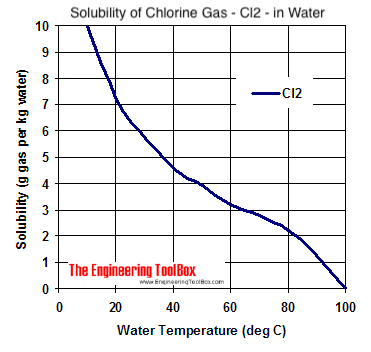
\includegraphics{assets/cl-solubility.png}
\end{figure}

% TODO: cite https://www.engineeringtoolbox.com/gases-solubility-water-d_1148.html

In this experiment, I attempt to determine the effectiveness of this approach by comparing the amounts of chlorine in tap water that has been boiled for different lengths of time. Through analyzing the data, I hope to find the optimal amount of time the water should be boiled for in order to remove a significant amount of chlorine.

To determine the amount of chlorine in a sample of tap water, Mohr's method will be used, which determines the chloride ion concentration in a solution by titrating it with silver nitrate. As silver nitrate is added to the solution, the chloride ions bond with the silver ions to create silver chloride:

\centerline{\ce{Ag^{+}_{(aq)} + Cl^{-}_{(aq) -> AgCl_{(s)}}}}


Hypochlorous acid has proven effective at inactivating deadly microbiological organisms like salmonella and E. coli, as well as many viruses. It is able to disrupt the cell membrane of these organisms and destroy their protein structures, ultimately ending in the cell's death.

While chlorine quickly reacts with inorganic compounds in water like ammonia and manganese, it takes longer to react with natural organic compounds like algal material. Thus, excess chlorine is often added at water treatment plants to ensure that the water remains disinfected throughout the distribution system and ultimately at our homes.

Yet, even at low concentrations, chlorine can still produce an unpleasant taste in water. One way that my family has been removing the undesirable taste of chlorine from our tap water by boiling it before using it. This works because the solubility of gases in liquids decreases with increasing temperature. Thus, as water is heated up, the amount of dissolved chlorine it holds decreases, and so the free chlorine is released in the form of chlorine gas.

% TODO: add theory, what would you do if you could increase the scope of the experiment

\section{Hypothesis}
Because chlorine is a gas at room temperature, boiling the water drives the gas out of the water.

\section{Variables}

\begin{table}[H]
	\def\arraystretch{1.5}
	\caption{A list of independent, dependent, and controlled variables during the experiment.}
	\begin{tabularx}{\linewidth}{|X|X|}
		\hline
		\multicolumn{2}{|c|}{\textbf{Independent Variable}}
		\\\hline
		Amount of time water is boiled  &
		TODO
		\\\hline
		\multicolumn{2}{|c|}{\centering \textbf{Dependent Variable}}
		\\\hline
		Amount of chlorine in water     &
		TODO
		\\\hline
		\multicolumn{2}{|c|}{\centering \textbf{Controlled Variables}}
		\\\hline
		Concentration of Silver Nitrate &
		TODO
		\\\hline
		Amount of water titrated        &
		TODO
		\\\hline
		Temperature of hot plate        &
		TODO
		\\\hline
	\end{tabularx}
\end{table}

\section{Apparatus}

<?#
I ended up using 2 mL total of 1 mol/L K2CrO4
This produces 0.01M

I remember using 0.01M of AgNO3 as well
?>

\begin{itemize}
	\item 50\ml Burette with 0.1\ml graduations
	\item Silver Nitrate
	\item 0.1\mpl Potassium Chromate Stock Solution
	\item 250\ml Erlenmeyer Flask for Titration
	\item 250\ml Beaker for Boiling water
	\item Hot Plate
	\item Burette stand
	\item 10\ml pipette
	\item Water deionizer (Thermo Scientific HN High Capacity Cartridge.)
	\item 100\ml graduated cylinder with 1\ml graduations for measuring water
	\item 10\ml graduated cylinder for creating \ce{K2CrO4} solution
	\item 100\ml graduated cylinder for creating 50\ml \ce{AgNO3} solution
	\item Analytical scale with $\pm$0.0001\gram precision
	\item Droppers
\end{itemize}

\section{Risk assessment}

Even though chlorine gas is released when tap water is boiled, the amount of chlorine released is so trace that it poses no appreciable danger. According to toronto.ca, the amount of chlorine in drinking water is regulated to be between 1 and \SI{3}{\mg\per\litre}, which is equal to 1 to 3 ppm. In addition, the experiment only involves boiling 100\ml of water at a time, which would only produce 0.1\mg to 0.3\mg of chlorine gas at a time, which according to ,
Even if all this free chlorine is released into the air, because the experiment is conducted in a large and ventilated room, the trace amount of chlorine gas released poses no threat as a health hazard.

\section{Procedure}

\begin{enumerate}
	\item A silver nitrate solution (\ce{AgNO3(aq)}) was created by measuring out 0.0817\g of solid \ce{AgNO3} and diluting it with 50\ml of deionized water.
	\item A dilute solution of 0.01\mpl \ce{K2CrO4} was created by measuring out 1\ml of the 0.1\mpl \ce{K2CrO4} stock solution and diluting it with 10\ml of deionized water.
	\item The \ce{AgNO3} solution was poured into a burette.
	\item 10\ml of tap water was transported into a 100\ml Erlenmeyer flask using a 10\ml pipette.
	\item Approximately 1\ml of the 0.01\mpl \ce{K2CrO4} solution was added to the 10\ml of tap water using a dropper.
	\item The initial volume of \ce{AgNO3} solution in the burette was noted down. The tap water was titrated with the \ce{AgNO3} solution until the solution turned reddish-brown (see Figure x). The final amount of solution in the burette was noted down.
	\item Steps 4 to 6 were repeated for 2-3 more trials.
	\item Steps 4 to 7 were repeated for deionized water and water boiled for 3, 6, 9, and 20 minutes using a hot plate.
\end{enumerate}

\section{Data}

% \begin{noindent}
<?
const silverNitrateSol = {
	mass: 0.0817,
	volume: 0.05,
	concentration: undefined,
};

/*
[0]: # of minutes boiled (or 'deionized' if the water was deionized)
[1]: mL of AgNO3 needed
[2]: mL of H2O used
*/

const rawData = [
	['deionized', 11.75 - 11.45, 10],
	['deionized', 31.15 - 30.8, 10],
	['deionized', 31.6 - 31.15, 10],
	[0, 11.45 - 10.15, 10],
	[0, 17.45 - 16.2, 10],
	[0, 18.7 - 17.45, 10],
	[3, 5.6 - 4.3, 10],
	[3, 14.3 - 13, 10],
	[3, 13 - 11.75, 10],
	[6, 20.15 - 18.7, 10],
	[6, 30.8 - 29.4, 10],
	[6, 7 - 5.6, 10],
	[9, 16.2 - 14.3, 10],
	[9, 10.15 - 8.65, 10],
	[20, 26.4 - 20.15, 10],
	[20, 29.4 - 26.4, 5],
];

const headers = ['minutesBoiled', 'titrantAmount', 'amountOfWater'];

const data = rawData.map(row => Object.fromEntries(R.zip(headers, row)));
?>
% \end{noindent}

\begin{table}[H]
	\caption{Data collected during the experiment over 16 trials. Note that the amount of water used for Trial 16 is only 5\ml because }
	\def\arraystretch{1.5}
	\begin{tabularx}{\linewidth}{|
			>{\RaggedRight}X|
			>{\RaggedRight}X|
			>{\RaggedRight}X|
			>{\RaggedRight}X|
		}
		\hline
		\textbf{Trial Number}                &
		\textbf{Time Boiled} /\si{\minute}   &
		\textbf{Titrant Amount} /$\pm$0.1\ml &
		\textbf{Amount of Water} /$\pm$0.05\ml
		\\\hline
		% \begin{noindent}
		<? for (const [rowIndex, row] of data.entries()) { ?>
			Trial <?= rowIndex + 1 ?>
			& <?= row.minutesBoiled ?>
			& <?= row.titrantAmount.toFixed(2) ?>
			& <?= row.amountOfWater ?>
			\\\hline
		<? } ?>
		% \end{noindent}
	\end{tabularx}
\end{table}

\section{Calculations}

To determine the concentration of chloride ions in the water, the amount of water and the amount of titrant is used.

The mass of \ce{AgNO3_{(s)}} used to create the silver nitrate solution was <?= silverNitrateSol.mass ?>\g. The analytical scale used to weigh this amount had an uncertainty of $\pm$0.0001\g. Using this information, the number of moles of silver nitrate in the solution can be determined:
%
\begin{align*}
	n_{\ce{AgNO3}} & = \frac{m_{\ce{AgNO3}}}{M_{\ce{AgNO3}}}
	\\
	n_{\ce{AgNO3}} & = \frac{(<?= silverNitrateSol.mass ?> \pm 0.0001)\g}{169.87\gpm}
	\\
	<? silverNitrateSol.moles = silverNitrateSol.mass / 169.87 -?>
	n_{\ce{AgNO3}} & = <?= sf(silverNitrateSol.moles, 3) ?>\mol \pm <?= sf(0.0001 / silverNitrateSol.mass * 100, 1) ?>\%
\end{align*}

The silver nitrate was diluted with 50\ml of deionized water using a graduated cylinder with an uncertainty of 0.5\ml or 1\%. Using the number of moles of \ce{AgNO3} in the solution, the concentration of the solution can be determined:
%
\begin{align*}
	c & = \frac{n}{V}
	\\
	c & = \frac{<?= sf(silverNitrateSol.moles, 3) ?>\mol \pm 0.1\%}{<?= silverNitrateSol.volume ?>\litre \pm 1\%}
	\\
	<? silverNitrateSol.concentration = silverNitrateSol.moles / silverNitrateSol.volume -?>
	c & = <?= sf(silverNitrateSol.concentration, 3) ?>\mpl \pm 1.1\%
\end{align*}

The concentration of the \ce{AgNO3} solution can then be used to determine the moles of \ce{AgNO3} for a given volume of the silver nitrate solution. For example, using the data in Trial 4, the volume of the silver nitrate solution needed to titrate the water was 1.30\ml $\pm$ 0.1\ml, or 1.30\ml $\pm$ 7.7\%, giving the following number of moles of \ce{AgNO3}:
%
\begin{align*}
	n & = V \times c
	\\
	n & = (1.30\ml \pm 7.7\%) \times (<?= sf(silverNitrateSol.concentration, 3) ?>\mpl \pm 1.1\%)
	\\
	<? const trial1Calculations = { molesOfSilverNitrate: silverNitrateSol.concentration * 1.30 } -?>
	n & = <?= sf(trial1Calculations.molesOfSilverNitrate, 3) ?>\mmol \pm 8.8\%
\end{align*}

The number of moles of \ce{AgNO3} can then be used to determine the number of moles of chloride ions in the water. The mole ratio between \ce{Ag^-} and \ce{Cl^-} can be determined from the reaction taking place between the silver nitrate and the chloride ions:

\centerline{\ce{AgNO3_{(aq)} + Cl^{-}_{(aq)} -> AgCl_{(s)} + NO3^{-}_{(aq)}}}

From the above balanced chemical equation, it can be determined that the mole ratio between \ce{Ag^-} and \ce{Cl^-} is 1. Therefore, the number of moles of \ce{AgNO3} is equal to the number of moles of \ce{Cl^-}:
%
\begin{align*}
	n_{\ce{Cl^-}} & = n_{\ce{AgNO3}}
	\\
	<? trial1Calculations.molesOfChlorine = trial1Calculations.molesOfSilverNitrate -?>
	n_{\ce{Cl^-}} & = <?= sf(trial1Calculations.molesOfChlorine, 3) ?>\mmol \pm 8.8\%
\end{align*}

From here, the concentration of chloride ions in the water can be determined knowing that the amount of water used was 10\ml $\pm$ 0.05\ml, or 10\ml $\pm$ 0.5\%:
%
\begin{align*}
	c & = \frac{<?= sf(trial1Calculations.molesOfChlorine, 3) ?>\mmol \pm 8.8\%}{10\mL \pm 0.5\%}
	\\
	c & = <?= sf(trial1Calculations.molesOfChlorine / 10, 3) ?>\mpl \pm 9\%
\end{align*}

The above calculations were performed for each of the values in the 16 trials, producing the following values:

% \begin{noindent}
<?
function calculateMolesOfChlorine(rowIndex: number) {
	const row = data[rowIndex];
	return row.titrantAmount * silverNitrateSol.concentration / row.amountOfWater;
}

function calculateMolesOfChlorineUncertaintyPercentage(rowIndex: number) {
	const row = data[rowIndex];
	const silverNitrateUncertaintyPercentage = 1.1;
	const titrantUncertaintyPercentage = (0.1 / row.titrantAmount) * 100;
	const amountOfWaterUncertaintyPercentage = 0.5;
	const totalUncertaintyPercentage =
		silverNitrateUncertaintyPercentage +
		titrantUncertaintyPercentage +
		amountOfWaterUncertaintyPercentage;
	return totalUncertaintyPercentage;
}

function formatFinalMolesOfChlorine(rowIndex: number) {
	const moles = calculateMolesOfChlorine(rowIndex);
	const uncertaintyPercentage = calculateMolesOfChlorineUncertaintyPercentage(rowIndex);
	return roundToUncertaintyDecimalPlaces(moles, uncertaintyPercentage);
}

function roundToUncertaintyDecimalPlaces(value: number, uncertaintyPercentage: number) {
	const uncertaintyString = sf(value * (uncertaintyPercentage / 100), 1);
	const decimalPlaces = uncertaintyString.length - uncertaintyString.indexOf('.') - 1;
	return `${value.toFixed(decimalPlaces)} $\\pm$ ${uncertaintyString}`;
}
?>
% \end{noindent}

\begin{table}[H]
	\caption{TODO}
	\def\arraystretch{1.5}
	\begin{tabularx}{\linewidth}{|
			>{\RaggedRight}X|
			>{\RaggedRight}X|
			>{\RaggedRight}X|
		}
		\hline
		\textbf{Time Boiled} /\si{\minute}
		 & \textbf{Concentration of \ce{Cl^-}} /\si{\mpl}
		 & \textbf{Average concentration of \ce{Cl^-}} /\si{\mpl}
		\\\hline
		% \begin{noindent}
		<? for (const [rowIndex, row] of data.entries()) { ?>
			<?= row.minutesBoiled ?>
			& <?= formatFinalMolesOfChlorine(rowIndex) ?>
			&
			<? if (row.minutesBoiled !== data[rowIndex - 1]?.minutesBoiled) { ?>
				<?
					const end = data.findIndex((dataRow, i) => i >= rowIndex && dataRow.minutesBoiled !== row.minutesBoiled);
					const trialIndexes = R.range(rowIndex, end === -1 ? data.length : end);
					const trialMoles = trialIndexes.map(
						(trialIndex) => calculateMolesOfChlorine(trialIndex)
					);
					const averageMolesOfChlorine = R.mean(trialMoles);
					const sumOfUncertaintyOfAverage = R.sum(trialIndexes.map(
						(trialIndex) =>
							calculateMolesOfChlorine(trialIndex) *
							(calculateMolesOfChlorineUncertaintyPercentage(trialIndex) / 100)
					));
					const uncertaintyPercentageOfAverage =
						sumOfUncertaintyOfAverage / R.sum(trialMoles) * 100
				?>
				\multirow{
					<?=
						R.count(
							(r) => r.minutesBoiled === row.minutesBoiled,
							data
						)
					?>
				}{*}{<?= roundToUncertaintyDecimalPlaces(averageMolesOfChlorine, uncertaintyPercentageOfAverage) ?>}
				\\\cline{1-2}
			<? } else if (row.minutesBoiled !== data[rowIndex + 1]?.minutesBoiled) { ?>
				\\\hline
			<? } else { ?>
				\\\cline{1-2}
			<? } ?>
		<? } ?>
		% \end{noindent}
	\end{tabularx}
\end{table}

\newpage

Plotting these values on a graph yields the following result:

\begin{figure}[H]
	\centering
	\caption{The concentration of chlorine remaining plotted against boiling time.}
	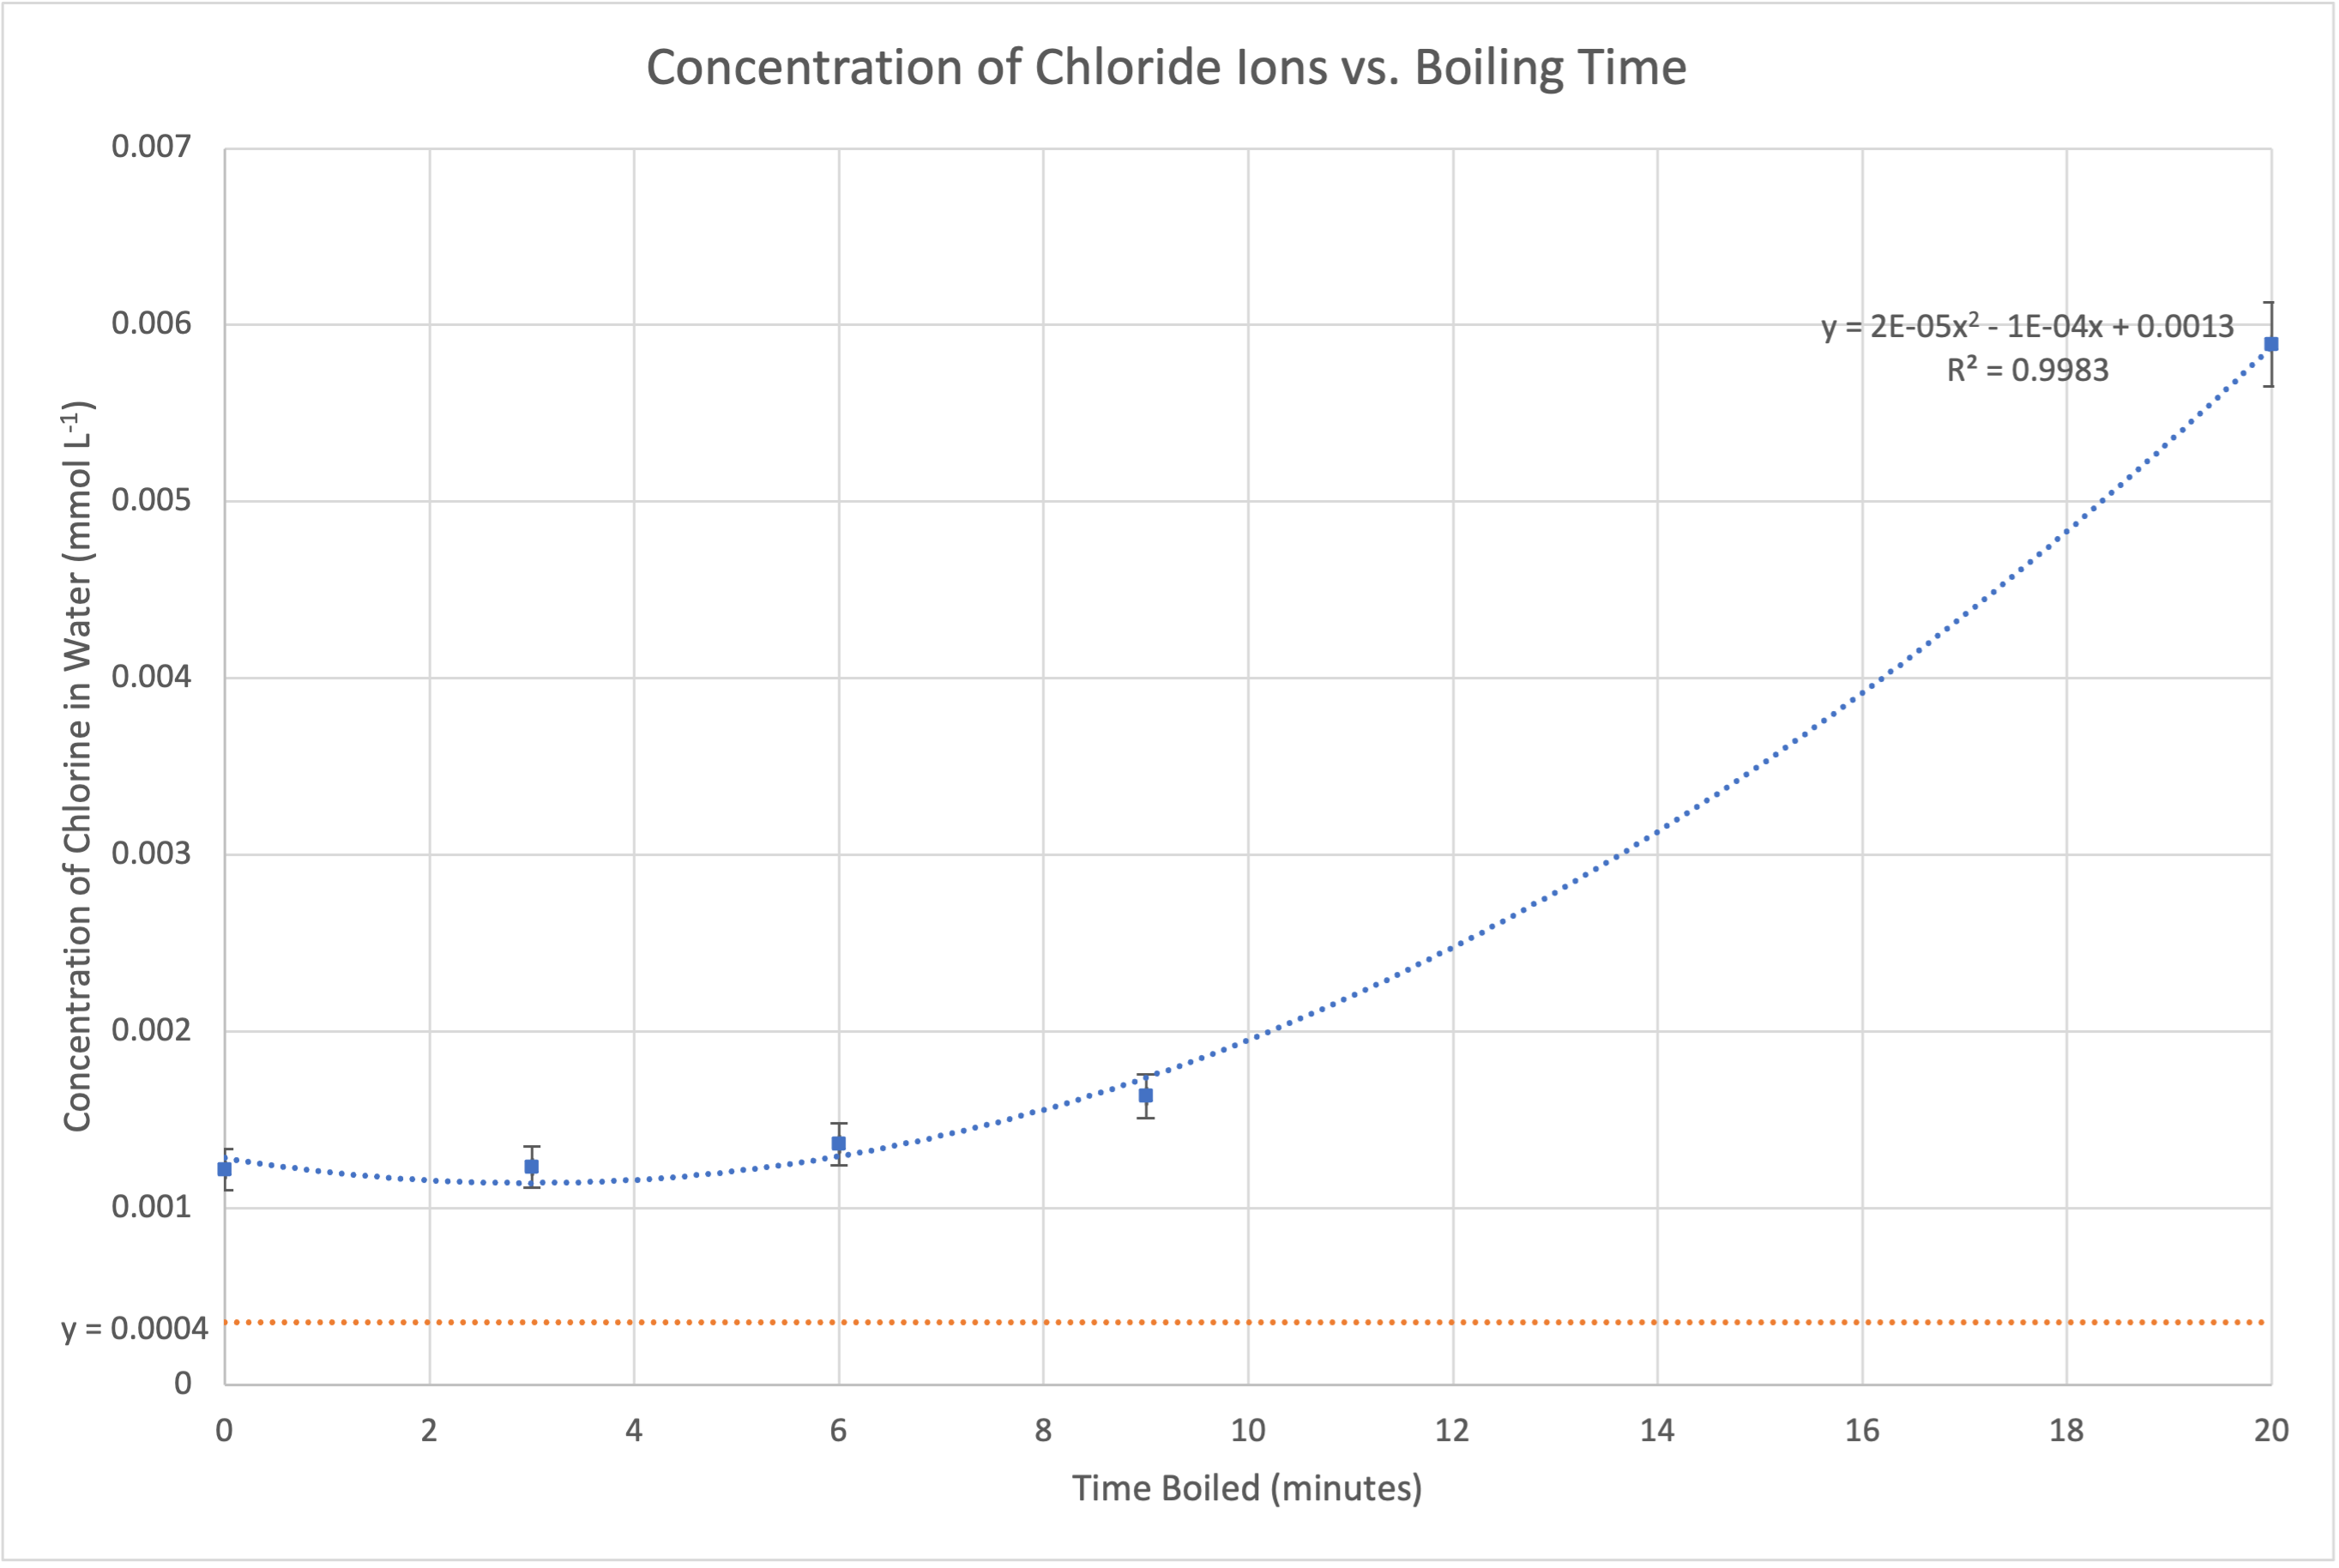
\includegraphics{assets/concentration-vs-boiling-time.png}
\end{figure}

\section{Analysis}

Based on the graph, the relationship between the amount of time the water was boiled for and the remaining chlorine in the water is quadratic. The equation of the trendline is as follows:
%
\begin{align*}
	y = 0.00002t^2 - 0.001t + 0.0013
\end{align*}

Where $y$ refers to the amount of chlorine remaining in the water sample (in \si{\mmol}) and where $t$ refers to the time the water has been boiled for (in \si{\minute}).

This graph goes against the hypothesis presented earlier, where it was predicted that the amount of chlorine remaining in the water should \textit{decrease} as the water was boiled for longer.

After conducting further research, it appears that the source of the water from the experiment (the high school's tap water) may have been disinfected with chloramine instead of chlorine. Unlike chlorine, boiling water containing chloramine.

This explanation is further supported by the effectiveness of the deionizer used in trials 1 to 3, which is represented by the red line in the graph. Unlike boiling, deionization is more effective at removing chloramine.

Thus, since boiling doesn't effectively remove chloramine, by boiling the water, the chloramine is still left in the water, making the water more concentrated with chlorine.

Thus, by boiling the water, it likely increased the concentration of chloramine and thus the chlorine concentration of the water, explaining the positive correlation between the time boiled and the amount of chlorine in the water.

Unfortunately, the final volume after boiling the water was not recorded (due to the expectation that it would be irrelevant to the experiment), limiting further analysis between the total amount of water remaining after boiling and the amount of chloramine remaining in the water.

% TODO: explain discrepancy in graph

% TODO: cite https://www.toronto.ca/311/knowledgebase/kb/docs/articles/toronto-water/water-treatment-and-supply/water-treatment-plants/f.j.-horgan-treatment-plant/reasons-that-the-city-uses-chlorine-to-treat-drinking-water.html
To verify the accuracy of this amount, the number of moles of chlorine can be compared to the recommended amount of chlorine concentration in drinking water: between 1\mg/\litre and 3\mg/\litre:
%
\begin{align*}
	m_{\ce{Cl^-}} & = n_{\ce{Cl^-}} \times M_{\ce{Cl^-}}
	\\
	M_{\ce{Cl^-}} & = 35.45\gpm
	\\
	m_{\ce{Cl^-}} & = <?= sf(trial1Calculations.molesOfChlorine, 3) ?> \pm 8.8\% \mmol \times 35.45\gpm
	\\
	<? trial1Calculations.massOfChlorine = trial1Calculations.molesOfSilverNitrate * 35.45 -?>
	m_{\ce{Cl^-}} & = <?= sf(trial1Calculations.massOfChlorine, 3) ?>\mg
\end{align*}

Converting this amount to \si{\mg\per\litre} gives us the following amount:
%
\begin{align*}
	c = <?= sf(trial1Calculations.massOfChlorine, 3) ?>\mg/10\ml
	\\
	c = <?= sf(trial1Calculations.massOfChlorine * 100, 3) ?>\mg/\litre
\end{align*}

This result is off by an order of magnitude: the experimental results indicate that there is over 10 times the amount of chlorine that is expected from tap water. The reason for this discrepancy is likely due to the low concentrations, A possible explanation for this is that the \ce{AgNO3} solution and \ce{K2CrO4} solutions were too dilute, so the initial colour change when all the \ce{AgNO3} ions had been formed was too faint to notice.

<?# add more possible reasons for this error ?>

\section{Conclusion}

While the results from this experiment may not have been accurate when compared to the expected amount of chlorine in Toronto's tap water, the data still displayed an evident trend between the amount of chlorine in water and the time the water was boiled for.


Through this trend, a conclusion that By plotting this trend and observing the positive correlation between, it can be concluded that the city of Toronto likely uses chloramine to disinfect their water.

Thus, since boiling water is not as effective in removing chloramine, my family should instead invest in a water filter or a reverse osmosis filter. <?# todo explain how those work ?>

\end{document}

% TODO: add 1 strength and many weaknesses
% TODO: past passive

% TODO: **specific** improvements (e.g. a specific instrument)